\documentclass[11pt]{article}
\usepackage{geometry,marginnote} % Pour passer au format A4
\geometry{hmargin=1cm, vmargin=1cm} % 

% Page et encodage
\usepackage[T1]{fontenc} % Use 8-bit encoding that has 256 glyphs
\usepackage[english,french]{babel} % Français et anglais
\usepackage[utf8]{inputenc} 

\usepackage{lmodern}
\setlength\parindent{0pt}

% Graphiques
\usepackage{graphicx,float,grffile}
\usepackage{pst-eucl, pst-plot,units} 

% Maths et divers
\usepackage{amsmath,amsfonts,amssymb,amsthm,verbatim}
\usepackage{multicol,enumitem,url,eurosym,gensymb}
\DeclareUnicodeCharacter{20AC}{\euro}

% Sections
\usepackage{sectsty} % Allows customizing section commands
\allsectionsfont{\centering \normalfont\scshape}

% Tête et pied de page

\usepackage{fancyhdr} 
\pagestyle{fancyplain} 

\fancyhead{} % No page header
\fancyfoot{}

\renewcommand{\headrulewidth}{0pt} % Remove header underlines
\renewcommand{\footrulewidth}{0pt} % Remove footer underlines

\newcommand{\horrule}[1]{\rule{\linewidth}{#1}} % Create horizontal rule command with 1 argument of height

%----------------------------------------------------------------------------------------
%   Début du document
%----------------------------------------------------------------------------------------

\begin{document}

\setlength{\columnseprule}{1pt}

\horrule{2px}
\section*{Chapitre 2 - Construire un triangle - \texttt{(G)}}
\horrule{2px}

Un triangle est une figure géométrique avec 3 côtés et 3 angles.

\section*{Peut-on toujours construire un triangle ?}

\subsection*{Avec n'importe quelle longueur ?}

Non... Si des côtés sont trop petits, ça ne marche pas.

\begin{figure}[H]
      \centering
      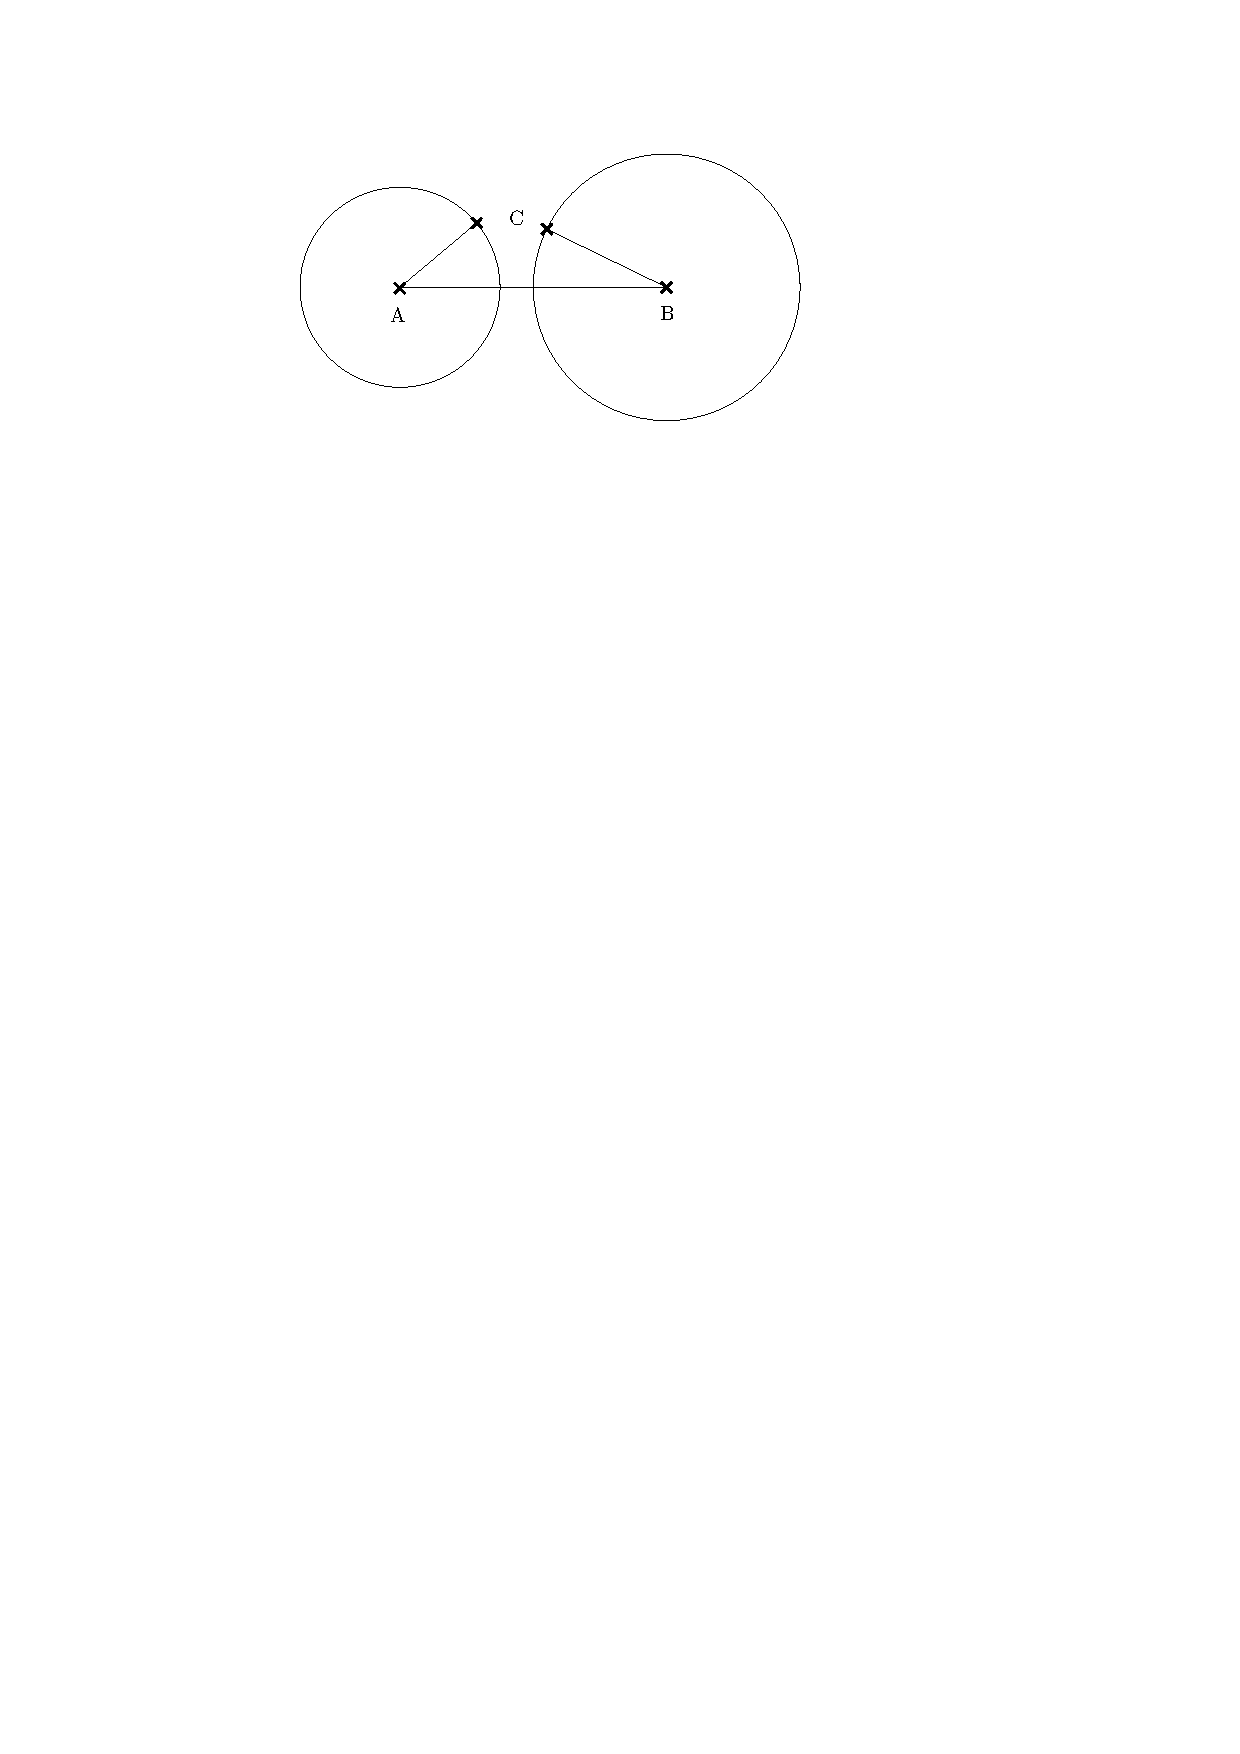
\includegraphics[width=0.7\linewidth]{5x2-triangles/sources/inegalite-triangulaire.pdf}
\end{figure}

\textsc{\textbf{L'inégalité triangulaire} : Pour construire un triangle, chaque côté du triangle doit être plus petit que la somme des deux autres.} 

Dans la pratique, on ne vérifiera que : \textsc{Le plus grand côté doit être plus petit que la somme des autres.} 

\paragraph*{Exercice type : Le triangle existe-t-il ?}~~\\

Soit ABC un triangle tel que AB = 12cm, BC = 6cm et AC = 22cm. \\ 
Peut-on construire le triangle ABC ?

Le plus grand côté est AC = 22cm.
\begin{align*}
  AB + BC &=& 12 + 6
  AB + BC &=& 18
\end{align*}

Donc $AB + BC < AC$
On ne peut pas construire le triangle. 

\subsection*{Avec n'importe quelle longueur ?}

On a envie de répondre non. On voit bien qu'on ne peut pas constuire un triangle avec trois angles droits...




\end{document}
